\chapter{Các giải thuật gom cụm}
\section{Giải thuật K-Means}
Vì giải thuật K-means khá đơn giản và có thể hữu hình hóa nên chúng ta sẽ đi
thẳng vào thuật toán để xem các bước thực hiện của giải thuật K-means như thế
nào, từ đó ta cũng có thể hiểu được cách tiếp cận vấn đề của giải
thuật.\\\\ 
 Các bước của giải thuật K-means được thực hiện theo trình tự:
\begin{enumerate}
  \item Gọi k là số cụm mong muốn, bắt đầu với việc chọn ngẫu nhiên các
  vector ``trọng tâm'' của k nhóm $\mu_1,\mu_2,\dots, \mu_k \in \mathbb{R} ^n $.
  \item Lặp cho đến khi hội tụ: \{ \\\\
  Với mỗi i, tính:
  \[ c^{(i)} := arg\:min_j||x^{(i)} - \mu_j||^2 \]
  Với mỗi j, tính:
  \[ \mu_j
  :=\frac{\sum_{i=1}^{m}1\{c^{(i)}=j\}x^{(i)}}{\sum_{i=1}^{m}1\{c^{(i)}=j\}}
  \]
  \}\\\\
  Dưới đây là hình mô phỏng cách thuật toán làm việc, với ví dụ điển hình là
  vector 2 chiều (Hình ảnh được trích từ CS229 Lecture Notes – 7a. The k-means
  clustering algorithm – Andrew Ng):\\\\\\\\\\\\
  \begin{figure}[h!]
  	\centering
	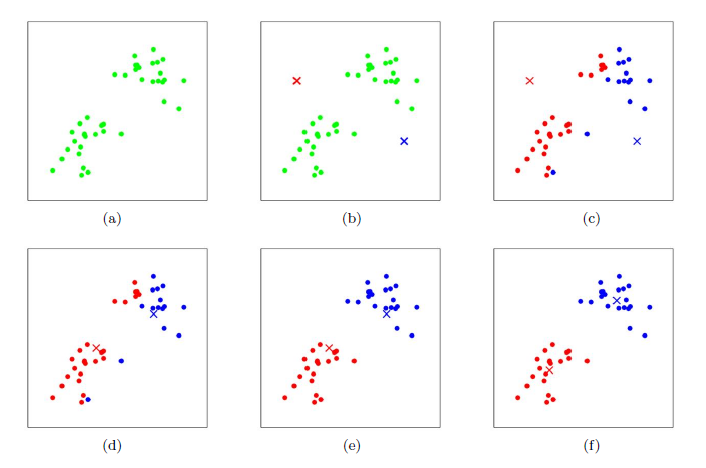
\includegraphics[width=7in,height=3in,keepaspectratio=true]{kmeans.png}
	\caption{Thuật toán K-means với vector 2 chiều}
  \end{figure}
  
  Giải thích hình trên:
  \begin{enumerate}
    \item Ta có tập dữ liệu đầu vào không nhãn, ta muốn chia tập dữ liệu
    này thành hai cụm.
    \item Ta chọn hai vector “trọng tâm” ban đầu bất kỳ, mỗi vector đại diện cho
    một cụm và được biễu diễn bằng điểm x trên đồ thị. Đây chính là bước (a) của thuật toán.
    \item Ở đây, ta giả sử vector “trọng tâm” nằm góc trên bên phải có giá trị
    $\mu_1$ đại diện cho nhãn $\{c^{(i)}=1\}$ và vector “trọng tâm” nằm góc dưới
    bên phải có giá trị $\mu_2$ đại diện cho nhãn $\{c^{(i)}=2\}$. Bắt đầu vào
    vòng lặp đầu tiên của bước (b). Thuật toán đi tính khoảng cách Euclid của
    tất cả các vector phần tử trong tập dữ liệu đến hai vector “trọng tâm”. Phần
    tử được đánh nhãn $\{c^{(i)}=1\}$ khi khoảng cách Euclid đến vector “trọng
    tâm” $\mu_1$ gần hơn so với vector “trọng tâm” $\mu_2$ hoặc ngược lại. Cứ
    tiếp tục như vậy ta sẽ gán nhãn cho tất cả các phần tử trong tập dữ liệu đầu vào.
    \item Ta cập nhật lại giá trị của vector “trọng tâm” bằng cách gán
    $\mu_j(j=1 \vee 2)$ bằng với giá trị trung bình của các phần tử thuộc nhãn
    do chính nó sở hữu. Đây chính là vòng lặp thứ 2 trong bước (b).
    \item Ta quay lại từ đầu của bước (b).
    \item Tiếp tục cập nhật cho đến khi hội tụ.
  \end{enumerate}
\end{enumerate}
\section{Giải thuật kết hợp Gaussian và EM (Mixture of Gaussians and
the EM Algorithm)}
Để giải quyết bài toán phân cụm, ta sẽ tiếp cận với một giải thuật dựa trên
nguyên lý của phân phối Gaussian và thuật toán EM – Expectation
Maximization.\\\\ 
Giả sử ta có bộ dữ liệu đầu vào được biểu diễn dưới dạng
$\{x^{(1)},\dots,x^{(m)}\}$, yêu cầu của bài toán là đưa ra kết quả với mỗi phần
tử trong tập dữ liệu được phân thành các cụm với các phần tử khác có “tính chất
tương tự nhau”. Lưu ý, tập dữ liệu của chúng ta không tồn tại nhãn.\\\\ 
Bắt đầu với “động lực” ban đầu của giải thuật, ta mong muốn chia tập dữ liệu
thành k nhóm và mỗi nhóm được đại diện bởi một mô hình phân phối xác suất. Ở
đây, nhận thấy mô hình phân phối Gaussian là thích hợp, vì giới hạn của báo cáo,
chúng ta sẽ khoan xem xét đến việc tại sao mô hình phân phối Gaussian được chọn?
Và nó thích hợp như thế nào? Mà thay vào đó sẽ đi làm rõ cách mà mô hình phân
hình Gaussian tham số hóa cho từng cụm dữ liệu của ta.\\\\ 
Xét xác suất $p(x^{(i)},z^{(i)}) = p(x^{(i)}|z^{(i)})p(z^{(i)})$. Trong công
thức này ta có $p(x^{(i)}|z^{(i)})$ là xác suất để phần tử $x^{(i)}$ thuộc vào
cụm được đánh nhãn $z^{(i)}$ và $p(z^{(i)})$ là xác suất để cụm được gán nhãn
$z^{(i)}$.\\\\ 
Từ cách giải thích đó, ta có được  $z^{(i)} \sim Multinomial(\phi
)$ (Multinominal – Phân phối đa thức) với $p(z^{(i)}=j)=\phi_j \geq 0,\:
\sum_{j-1}^{k}\phi_j =1$, và $(x^{(i)}|z^{(i)} =j)\sim
\mathcal{N}(\mu_j,\Sigma_j)$.\\\\ 
Mặc khác, như đã nó bên trên, vì $(x^{(i)}|z^{(i)} =j)\sim
\mathcal{N}(\mu_j,\Sigma_j)$ nên ta có thể viết lại xác suất ban đầu dưới dạng
phụ thuộc vào $\mu_j,\:\Sigma_j$:
\[ p(x^{(i)},z^{(i)}) = p(x^{(i)};\:\phi,\:\mu,\:\Sigma) \]
Tiếp tục phân tích:
\[ p(x^{(i)};\:\phi,\:\mu,\:\Sigma) = \sum_{z^{(i)}=1}^{k}
p(x^{(i)}|z^{(i)};\:\mu,\:\Sigma)p(z^{(i)};\:\phi) \] 
Tại đây ta thấy được bài toán thực sự được sử dụng Mixtures of Gaussian như thế
nào vào việc mô hình hóa.\\\\
Công việc tiếp theo chúng ta sẽ đi cực đại giá trị xác suất
$p(x^{(i)};\:\phi,\:\mu,\:\Sigma)$ cho từng cụm – vì ta giả sử có k cụm nên việc này đồng nghĩa ta phải cực đại cho k xác suất như
vậy. Việc này cũng có ý nghĩa là, khi ta xét một phần tử bất kỳ ta sẽ đi tính
xác suất của điểm này cho k cụm, nghĩa là thử nó với từng mô hình xác suất, và
nó sẽ được kết luận thuộc cụm có giá trị xác suất là cao nhất.\\\\ 
Để giải quyết bài toán cực đại ta sử dụng thuật toán Maximum Likelihood. Ta có
biểu thức likelihood của xác suất ban đầu với m là số phần tử của tập đầu vào:
\[ l(\phi,\:\mu,\:\Sigma) = \sum_{i=1}^{m} \log\:
p(x^{(i)};\:\phi,\:\mu,\:\Sigma) = \sum_{i=1}^{m} \log \sum_{z^{(i)}=1}^{k}
p(x^{(i)}|z^{(i)};\:\mu,\:\Sigma)p(z^{(i)};\:\phi) \]
Tạm dừng bài toán tại đây. Chúng ta sẽ chuyển sang Giải thuật EM, để cung cấp
cho chúng ta một công cụ có thể giúp tiếp tục giải quyết bài toán.\\\\ 
Định nghĩa hàm lồi – lõm: Hàm f được gọi là lồi khi $f'' \geq 0$. Ngược lại, 
$f'' \leq 0$ thì f được gọi là hàm lõm.\\\\ 
Bất đẳng thức Jensen: Cho hàm lồi f, với bất kỳ X ta luôn có:
\[ E[f(X)] \geq f[E(X)] \]
Điều kiện đẳng thức xảy ra khi $X=E[X]$\\\\
Ta có thể suy rộng ra cho trường hợp f là hàm lõm, dấu của bất đẳng thức sẽ được
đảo chiều:
\[ E[f(X)] \leq f[E(X)] \]
Điều kiện đẳng thức vẫn giữ nguyên.\\\\ 
Xét $f(x) = \log(x)$ và $x=\frac{p(x^{(i)},z^{(i)};\theta)}{Q_i(z^{(i)})} $ .
Khoan hãy nghi vấn tại sao chúng ta đặt như vậy mà hãy xem phép biến đổi dưới đây để hiểu rõ hơn:
\begin{align} \sum_{i} \log\: p(x^{(i)};\:\theta) & = \sum_{i} \log
\sum_{z^{(i)}} p(x^{(i)},z^{(i)};\:\theta) = \sum_{i} \log \sum_{z^{(i)}}
Q_i(z^{(i)})\frac{p(x^{(i)},z^{(i)};\:\theta)}{Q_i(z^{(i)})}  \notag \\
& \geq \sum_{i} \sum_{z^{(i)}}
Q_i(z^{(i)})\:\log \frac{p(x^{(i)},z^{(i)};\:\theta)}{Q_i(z^{(i)})} \notag
\end{align}
Tới đây, ta thấy được việc đặt ở trên để đưa về dạng chuẩn của bất đẳng thức
Jensen cho hàm lõm.\\\\ 
Bây giờ ta đã có đầy đủ công cụ để giải quyết tiếp bài toán ban đầu.\\\\ 
Ta đa dừng lại ở việc phải đi cực đại biểu thức Likelihood:
\[ l(\phi,\:\mu,\:\Sigma) = \sum_{i=1}^{m} \log\:
p(x^{(i)};\:\phi,\:\mu,\:\Sigma) = \sum_{i=1}^{m} \log \sum_{z^{(i)}=1}^{k}
p(x^{(i)}|z^{(i)}=j;\:\mu,\:\Sigma)p(z^{(i)=j};\:\phi) \]
Với $w_{j}^{(i)} = P(z^{(i)}=j|x^{(i)};\:phi,\:\mu,\:\Sigma)$, ta có:
\begin{multline}
\sum_{i=1}^{m} \log \sum_{z^{(i)}=1}^{k}
p(x^{(i)}|z^{(i)};\:\mu,\:\Sigma)p(z^{(i)};\:\phi) = \sum_{i=1}^{m} \log
\sum_{j=1}^{k}
w_{j}^{(i)}\frac{p(x^{(i)}|z^{(i)};\:\mu,\:\Sigma)p(z^{(i)};\:\phi)}{w_{j}^{(i)}}\\
\geq \sum_{i=1}^{m} \sum_{j=1}^{k} w_{j}^{(i)} \log
\frac{\frac{1}{(2\pi)^{n/2}|\Sigma_j|^{1/2}}\exp\left( -\frac{1}{2}
(x^{(i)}-\mu_j)^T \Sigma_j^{-1} (x^{(i)}-\mu_j)
\right).\phi_j}{w_{j}^{(i)}}\notag
\end{multline}
Để cực đại biểu thức bên phải, chúng ta thực hiện bằng cách đạo hàm từng phần
lần lượt với $\mu$, $\phi$ và $\Sigma$ sau đó đặt bằng 0, từ biểu thức thu được
ta giải nghiệm.\\\\ 
Bắt đầu với đạo hàm riêng theo $\mu_l$ với $l=1,\dots, k$
\begin{align}
\nabla_{u_l} & \sum_{i=1}^{m} \sum_{j=1}^{k} w_{j}^{(i)} \log
\frac{\frac{1}{(2\pi)^{n/2}|\Sigma_j|^{1/2}}\exp\left( -\frac{1}{2}
(x^{(i)}-\mu_j)^T \Sigma_j^{-1} (x^{(i)}-\mu_j)
\right).\phi_j}{w_{j}^{(i)}}\notag\\
& =  \nabla_{u_l} \sum_{i=1}^{m} \sum_{j=1}^{k} w_{j}^{(i)} \left( \log
\frac{\frac{1}{(2\pi)^{n/2}|\Sigma_j|^{1/2}}\phi_j }{w_{j}^{(i)}} -\frac{1}{2}
(x^{(i)}-\mu_j)^T \Sigma_j^{-1} (x^{(i)}-\mu_j) \right)\notag\\
& = \nabla_{u_l} \sum_{i=1}^{m} \sum_{j=1}^{k} w_{j}^{(i)} \log
\frac{\frac{1}{(2\pi)^{n/2}|\Sigma_j|^{1/2}}\phi_j }{w_{j}^{(i)}} -\frac{1}{2}
\nabla_{u_l} \sum_{i=1}^{m} \sum_{j=1}^{k} w_{j}^{(i)} (x^{(i)}-\mu_j)^T
\Sigma_j^{-1} (x^{(i)}-\mu_j)\notag\\
& = -\frac{1}{2} \nabla_{u_l} \sum_{i=1}^{m} \sum_{j=1}^{k} w_{j}^{(i)}
(x^{(i)}-\mu_j)^T \Sigma_j^{-1} (x^{(i)}-\mu_j)\notag\\
& = -\frac{1}{2} \sum_{i=1}^{m} \nabla_{u_l} \sum_{j=1}^{k} w_{j}^{(i)}
(x^{(i)}-\mu_j)^T \Sigma_j^{-1} (x^{(i)}-\mu_j)\notag\\
& = -\frac{1}{2} \sum_{i=1}^{m} \nabla_{u_l} w_{l}^{(i)}
(x^{(i)}-\mu_l)^T \Sigma_l^{-1} (x^{(i)}-\mu_l)\notag\\
& = -\frac{1}{2} \sum_{i=1}^{m} w_{l}^{(i)} \nabla_{u_l} 
(x^{(i)^T}-\mu_l^T) \Sigma_l^{-1} (x^{(i)}-\mu_l)\notag\\
& = -\frac{1}{2} \sum_{i=1}^{m} w_{l}^{(i)} \nabla_{u_l} (x^{(i)^T} \Sigma_l^{-1}
x^{(i)} - \mu_l^T \Sigma_l^{-1} x^{(i)} - x^{(i)^T} \Sigma_l^{-1} \mu_l + \mu_l^T
\Sigma_l^{-1} \mu_l)\notag\\
& = -\frac{1}{2} \sum_{i=1}^{m} w_{l}^{(i)} \nabla_{u_l} (- \mu_l^T \Sigma_l^{-1}
x^{(i)} - x^{(i)^T} \Sigma_l^{-1} \mu_l + \mu_l^T
\Sigma_l^{-1} \mu_l)\notag\\
& = \frac{1}{2} \sum_{i=1}^{m} w_{l}^{(i)} \nabla_{u_l} ( \mu_l^T \Sigma_l^{-1}
x^{(i)} + x^{(i)^T} \Sigma_l^{-1} \mu_l - \mu_l^T
\Sigma_l^{-1} \mu_l)\notag\\
& = \frac{1}{2} \sum_{i=1}^{m} w_{l}^{(i)} \nabla_{u_l} tr( \mu_l^T \Sigma_l^{-1}
x^{(i)} + x^{(i)^T} \Sigma_l^{-1} \mu_l - \mu_l^T
\Sigma_l^{-1} \mu_l)\notag\\
& = \frac{1}{2} \sum_{i=1}^{m} w_{l}^{(i)} \nabla_{u_l} (tr(\mu_l^T \Sigma_l^{-1}
x^{(i)}) + tr(x^{(i)^T} \Sigma_l^{-1} \mu_l) - tr(\mu_l^T
\Sigma_l^{-1} \mu_l))\notag\\
& = \frac{1}{2} \sum_{i=1}^{m} w_{l}^{(i)} \nabla_{u_l} (tr(\mu_l^T \Sigma_l^{-1}
x^{(i)}) + tr(x^{(i)^T} \Sigma_l^{-1} \mu_l)^T - tr(\mu_l^T
\Sigma_l^{-1} \mu_l))\notag\\
& = \frac{1}{2} \sum_{i=1}^{m} w_{l}^{(i)} \nabla_{u_l} (2tr(\mu_l^T \Sigma_l^{-1}
x^{(i)}) - tr(\mu_l^T \Sigma_l^{-1} \mu_l))\notag\\
& = \frac{1}{2} \sum_{i=1}^{m} w_{l}^{(i)} \nabla_{u_l} (2(\mu_l^T \Sigma_l^{-1}
x^{(i)}) - (\mu_l^T \Sigma_l^{-1} \mu_l))\notag\\
& = \sum_{i=1}^{m} w_{l}^{(i)} (\Sigma_l^{-1}
x^{(i)} - \Sigma_l^{-1} \mu_l)\notag
\end{align}
Đặt $\sum_{i=1}^{m} w_{l}^{(i)} (\Sigma_l^{-1}
x^{(i)} - \Sigma_l^{-1} \mu_l) = 0$. Giải phương trình ta được:
\[ \mu_l = \frac{\sum_{i=1}^{m} w_l^{(i)} x^{(i)}}{\sum_{i=1}^{m} w_l^{(i)}} \]
Tiếp tục với đạo hàm riêng theo $\phi_j$. Ta nhận thấy biểu thức chỉ có một biến
duy nhất phụ thuộc vào $\phi_j$ , ta dễ dàng viết được:
\begin{align} \nabla_{\phi_j} \sum_{i=1}^{m} \sum_{j=1}^{k} w_{j}^{(i)} & \log
\frac{\frac{1}{(2\pi)^{n/2}|\Sigma_j|^{1/2}}\exp\left( -\frac{1}{2}
(x^{(i)}-\mu_j)^T \Sigma_j^{-1} (x^{(i)}-\mu_j)
\right).\phi_j}{w_{j}^{(i)}}\notag\\
& =  \nabla_{\phi_j} \sum_{i=1}^{m} \sum_{j=1}^{k} w_{j}^{(i)} \log \phi_j\notag
\end{align}
Điều này đồng nghĩa với việc bài toán cực đại ban đầu theo $\phi_j$ sẽ tương ứng
với việc đi cực đại $\sum_{i=1}^{m} \sum_{j=1}^{k} w_{j}^{(i)} \log \phi_j$ theo
$\phi_j$.\\\\
Tuy nhiên, $\phi_j$ chịu ràng buộc $\sum_{j=1}^{k} \phi_j=1$ nên ta cần dùng đến
kỹ thuật Lagrangian:\\\\
Đặt:
\[ \mathcal{L}(\phi)= \sum_{i=1}^{m} \sum_{j=1}^{k} w_{j}^{(i)} \log \phi_j +
\beta \left( \sum_{j=1}^{k} \phi_j-1 \right) \]
Để cực đại $\mathcal{L}(\phi)$ ta đơn giản chi đi đạo hàm riêng theo $\phi_j$
\[ \frac{\partial}{\partial\phi_j}\mathcal{L}(\phi)= \sum_{i=1}^m
\frac{w_j^{(i)}}{\phi_j} + \beta \]
Giải phương trình $\sum_{i=1}^m \frac{w_j^{(i)}}{\phi_j}
+ \beta = 0$ ra được $\phi_j = -\frac{1}{\beta}\sum_{i=1}^m w_j^{(i)}$.\\\\
Ta nhận thấy:
\[ \phi_j = -\frac{1}{\beta}\sum_{i=1}^m w_j^{(i)} \Rightarrow \sum_{j=1}^{k}
\phi_j = -\frac{1}{\beta} \sum_{j=1}^{k} \sum_{i=1}^m w_j^{(i)} \]
Mặt khác:
\[ \sum_{j=1}^{k} \phi_j = 1 \Rightarrow -\beta = \sum_{j=1}^{k}
\sum_{i=1}^m w_j^{(i)} = \sum_{i=1}^m 1 = m \]
Vậy:
\[ \phi_j = \frac{1}{m} \sum_{i=1}^m w_j^{(i)} \]
Cuối cùng với đạo hàm riêng theo $\Sigma_l$ . Tuy nhiên việc đạo hàm riêng theo
$\Sigma_l$ sẽ dẫn đến các biến đổi toán học phức tạp. Tiếp cận với một hướng khác, ta đạo hàm riêng
theo $\Sigma_l^{-1}$, việc này vẫn giữ được bản chất vấn đề nhưng lại dẫn đến các
biến đổi toán học dễ dàng hơn so với hướng tiếp cận ban đầu.
\begin{align}
\nabla_{\Sigma_l^{-1}} & \sum_{i=1}^{m} \sum_{j=1}^{k} w_{j}^{(i)} \log
\frac{\frac{1}{(2\pi)^{n/2}|\Sigma_j|^{1/2}}\exp\left( -\frac{1}{2}
(x^{(i)}-\mu_j)^T \Sigma_j^{-1} (x^{(i)}-\mu_j)
\right).\phi_j}{w_{j}^{(i)}}\notag\\
& = \sum_{i=1}^{m} w_{j}^{(i)} \nabla_{\Sigma_l^{-1}} \left( \log
\frac{\frac{1}{(2\pi)^{n/2}|\Sigma_l|^{1/2}}\phi_l }{w_{l}^{(i)}} -\frac{1}{2}
(x^{(i)}-\mu_l)^T \Sigma_l^{-1} (x^{(i)}-\mu_l) \right)\notag
\end{align}
Đặt:
\begin{align}
\sum_{i=1}^{m} w_{j}^{(i)} \nabla_{\Sigma_l^{-1}} \log
\frac{\frac{1}{(2\pi)^{n/2}|\Sigma_l|^{1/2}}\phi_l }{w_{l}^{(i)}}\\
\sum_{i=1}^{m} w_{j}^{(i)} \nabla_{\Sigma_l^{-1}} \left( -\frac{1}{2}
(x^{(i)}-\mu_l)^T \Sigma_l^{-1} (x^{(i)}-\mu_l) \right)
\end{align}
Biến đổi (4.1):
\begin{align}
(4.1)& = \sum_{i=1}^{m} w_{j}^{(i)} \nabla_{\Sigma_l^{-1}} \left( \log
\frac{\frac{1}{(2\pi)^{n/2}}\phi_l }{w_{l}^{(i)}} - \log |\Sigma_l|^{1/2} \right)
= \sum_{i=1}^{m} w_{j}^{(i)} \nabla_{\Sigma_l^{-1}} \left( -\log |\Sigma_l|^{1/2}
\right)\notag\\
& = -\frac{1}{2} \sum_{i=1}^{m} w_{j}^{(i)} \nabla_{\Sigma_l^{-1}} -\log
|\Sigma_l| = -\frac{1}{2} \sum_{i=1}^{m} w_{j}^{(i)} \nabla_{\Sigma_l^{-1}} -\log
\frac{1}{|\Sigma_l^{-1}|}\notag\\ 
& = -\frac{1}{2} \sum_{i=1}^{m} w_{j}^{(i)}
\frac{\nabla_{\Sigma_l^{-1}}
\frac{1}{|\Sigma_l^{-1}|}}{\frac{1}{|\Sigma_l^{-1}|}} = \frac{1}{2} \sum_{i=1}^{m}
w_{j}^{(i)} \frac{\frac{\nabla_{\Sigma_l^{-1}}
\sum^{-1}}{|\Sigma_l^{-1}|^2}}{\frac{1}{|\Sigma_l^{-1}|}}\notag\\ 
& = \frac{1}{2}
\sum_{i=1}^{m} w_{j}^{(i)} \frac{|\Sigma_l^{-1}||\Sigma_l|^T}{|\Sigma_l^{-1}|} = \frac{1}{2}
\sum_{i=1}^{m} w_{j}^{(i)}\Sigma_l^T = \frac{1}{2}
\sum_{i=1}^{m} w_{j}^{(i)}|\Sigma_l|\notag
\end{align}
Trước khi bước vào việc biến đổi (4.2) ta cần đi chứng minh một bổ đề:
Với x là vector n chiều và A là ma trận $(n\times n)$ thì
$\nabla_A(x^T.Ax)=x.x^T$\\
Thật vậy:
\begin{align}
x & = 
\begin{bmatrix}
x_1 \\ \vdots \\ x_n
\end{bmatrix};\quad 
x^T = 
\begin{bmatrix}
x_1 & \dots & x_n
\end{bmatrix};\quad 
A = 
\begin{bmatrix}
A_{11} & \dots & A_{1n}\\ 
\vdots & \ddots & \vdots\\ 
A_{n1} & \dots & A_{nn}
\end{bmatrix}\notag\\
& x^TAx  = 
\begin{bmatrix}
x_1 & \dots & x_n
\end{bmatrix} 
\begin{bmatrix}
A_{11} & \dots & A_{1n}\\ 
\vdots & \ddots & \vdots\\ 
A_{n1} & \dots & A_{nn}
\end{bmatrix}
\begin{bmatrix}
x_1 \\ \vdots \\ x_n
\end{bmatrix}\notag\\
& = 
\begin{bmatrix}
x_1A_{11} + \dots + x_nA_{n1} & x_1A_{12} + \dots + x_nA_{n2} & \dots &
x_1A_{1n} + \dots + x_nA_{nn}
\end{bmatrix} 
\begin{bmatrix}
x_1 \\ \vdots \\ x_n
\end{bmatrix}\notag\\
& = (x_1A_{11}x_1 + \dots + x_nA_{n1}x_1) + (x_1A_{12}x_2 + \dots + x_nA_{n2}x_2) +
\dots \notag\\ & + (x_1A_{1n}x_n + \dots + x_nA_{nn}x_n)\notag\\
& = \sum_{i=1}^{n} \sum_{j=1}^{n} x_iA_{ij}x_j = F\notag
\end{align}
Suy ra:
\[ \nabla_A(x^TAx) = \nabla_AF = 
\begin{bmatrix}
  \frac{\partial f}{\partial A_{11}} & \dots & \frac{\partial f}{\partial
  A_{1n}}\\
  \vdots & \ddots & \vdots \\
  \frac{\partial f}{\partial A_{n1}} & \dots & \frac{\partial f}{\partial
  A_{nn}}  
   \end{bmatrix}
 = 
\begin{bmatrix}
x_1x_1 & \dots & x_1x_n\\ 
\vdots & \ddots & \vdots\\ 
x_nx_1 & \dots & x_nx_n
\end{bmatrix}
= x.x^T
 \]
 Từ bổ đề trên ta biến đổi (4.2):
\[ (4.2) = -\frac{1}{2} \sum_{i=1}^{m} w_{j}^{(i)} \nabla_{\Sigma_l^{-1}} \left( 
(x^{(i)}-\mu_l)^T \Sigma_l^{-1} (x^{(i)}-\mu_l) \right) = -\frac{1}{2} \sum_{i=1}^{m} w_{j}^{(i)} \left( 
(x^{(i)}-\mu_l) (x^{(i)}-\mu_l)^T \right) \]
Kết hợp (4.1) và (4.2) sau biến đổi:
\begin{align}
\nabla_{\Sigma_l^{-1}} & \sum_{i=1}^{m} \sum_{j=1}^{k} w_{j}^{(i)} \log
\frac{\frac{1}{(2\pi)^{n/2}|\Sigma_j|^{1/2}}\exp\left( -\frac{1}{2}
(x^{(i)}-\mu_j)^T \Sigma_j^{-1} (x^{(i)}-\mu_j)
\right).\phi_j}{w_{j}^{(i)}} = (4.1) + (4.2) \notag\\
& = \frac{1}{2} \sum_{i=1}^{m} w_{j}^{(i)} |\Sigma_l| -\frac{1}{2} \sum_{i=1}^{m}
w_{j}^{(i)} \left( (x^{(i)}-\mu_l) (x^{(i)}-\mu_l)^T \right)\notag
\end{align}
Đặt biểu thức trên bằng 0 và giải phương trình theo $\Sigma$ suy ra:
\[ \Sigma_j = \frac{\sum_{i=1}^{m}
w_{j}^{(i)} \left( (x^{(i)}-\mu_j) (x^{(i)}-\mu_l)^T \right)}{\sum_{i=1}^{m}
w_{j}^{(i)}} \]
Từ việc cực đại bằng phương pháp lấy đạo hàm riêng ta được kết quả cuối cùng:
\begin{align}
& \phi_j = \frac{1}{m}\sum_{i=1}^m w_j^{(i)},\notag\\
& \mu_j = \frac{\sum_{i=1}^m w_j^{(i)} x^{(i)}}{\sum_{i=1}^m
w_j^{(i)}},\notag\\
& \Sigma_j = \frac{\sum_{i=1}^m w_j^{(i)} (x^{(i)}-\mu_j)
(x^{(i)}-\mu_j)^T}{\sum_{i=1}^m w_j^{(i)}}\notag
\end{align}
Từ kết quả này ta đưa ra các bước lặp cho giải thuật Mixtures of Gaussian và
EM.\\\\
Lặp cho đến khi hội tụ: \{\\
\tab (E-step) Với mỗi i, j, tính:
\[ w_j^{(i)} := p(z^{(i)} = j \vee x^{(i)}; \phi,\:\mu,\:\Sigma) \]
\tab (M-step) Cập nhật thông số:
\begin{align}
& \phi_j = \frac{1}{m}\sum_{i=1}^m w_j^{(i)},\notag\\
& \mu_j = \frac{\sum_{i=1}^m w_j^{(i)} x^{(i)}}{\sum_{i=1}^m
w_j^{(i)}},\notag\\
& \Sigma_j = \frac{\sum_{i=1}^m w_j^{(i)} (x^{(i)}-\mu_j)
(x^{(i)}-\mu_j)^T}{\sum_{i=1}^m w_j^{(i)}}\notag
\end{align}
\}
\section{Giải thuật Self Organizing Maps - SOM}
\subsection{Giới thiệu}
SOM là một giải thuật dựa trên mô hình học không giám sát (unsupervised
learning), trong đó các hình thành một bản đồ để tạo thành phân loại riêng về dữ
liệu huấn luyện mà không cần sự giúp đỡ từ bên ngoài. Để làm điều này chúng ta
phải giả định rằng các thành viên lớp được định nghĩa rộng của các mô hình đầu
vào chia sẻ các tính năng phổ biến (common features), và rằng mạng sẽ có thể xác
định những tính năng trên phạm vi của mô hình đầu vào.\\\\ 
 Một phần đặc biệt thú vị của hệ thống unsupervised được dựa trên competitive
 learning, trong đó các neuron ra cạnh tranh với nhau để được kích hoạt, với kết
 quả là chỉ có một được kích hoạt tại bất kỳ thời điểm nào. Neuron kích hoạt này
 được gọi là winner-takes-all neuron hoặc chỉ đơn giản là neuron chiến thắng
 (winning neuron) hay Best Matching Unit (BMU). Cạnh tranh như vậy có thể được
 thực hiện bằng cách kết nối biên (lateral inhibition connections - đường dẫn
 thông tin phản hồi tiêu cực) giữa các neuron. Không chỉ vậy mà winning neuron
 còn tác động đến các neuron xung quanh nó. Kết quả là các neuron bị buộc phải
 tự tổ chức. Vì thế nên được gọi là tự tổ chức Self Organizing Map
 (SOM).\\\\ 
 Làm thế nào chúng ta có thể thực hiện đưa các thuộc tính vào trong
 unsupervised. Điều đầu tiên để nhận ra là ta cần một số tương tác giữa các
 neuron trong mạng, do đó, khi một neuron hoạt động, nó ảnh hưởng đến những
 neuron xung quanh. Làm thế nào để sự tương tác này làm việc? Neuron gần nhau
 trong mô hình đại diện cho các thuộc tính tương tự. Điều này có nghĩa rằng các
 winning neuron nên kéo neuron khác gần với nó trong mạng gần hơn với bản thân
 trong không gian trọng số. Tương tự như vậy, neuron ở xa đại diện thuộc tính
 khác nhau, do đó winning neuron đẩy các neuron đó đi bằng cách sử dụng các kết
 nối tiêu cực Neuron mà rất xa trong mạng đại diện cho các thuộc tính khác với
 winning neuron, vì vậy chỉ cần bỏ qua chúng.
\subsection{Thành phần của SOM}
Mục tiêu chính của một SOM là biến đổi một mô hình không gian nhiều chiều thành
mô hình có một hoặc hai chiều rời rạc.\\\\
Do đó thiết lập SOM bằng cách đặt các neuron tại các nút của lưới một hoặc hai
chiều. Bản đồ có nhiều chiều hơn có thể thực hiện được nhưng không được sử dụng
nhiều.\\\\
Các neuron chọn lọc để điều chỉnh mô hình đầu vào khác nhau (kích thích) hoặc
các lớp của mô hình đầu vào trong quá trình học tập cạnh tranh.\\\\
Vị trí của các neuron để điều chỉnh trở nên có trật tự và một hệ thống phối hợp
có ý nghĩa cho các đầu vào các tính năng được tạo ra trên mạng. SOM do đó tạo
thành bản đồ cần thiết của mô hình đầu vào.\\\\ 
Chúng ta có thể xem đây là một sự tổng quát phi tuyến phân tích thành phần chính
(PCA).
  \subsubsection{Kiến trúc SOM}
  Một kiến trúc mạng neuron dựa trên học tập cạnh tranh phát minh bởi Teuvo
  Kohonen năm 1981. Không phụ thuộc vào sự lựa chọn ưu tiên của số cụm để tìm
  kiếm - sẽ tìm thấy số lượng các cụm thích hợp cho các bộ instances.  Đôi khi
  được coi là không gian hai chiều của cụm trong không gian nhiều
  chiều.\\ 
  SOM có một cấu trúc feed-forward với một lớp tính toán đơn
  sắp xếp thành hàng và cột. Mỗi neuron được kết nối đầy đủ với tất cả các nút nguồn trong lớp nhập:\\ 
  \begin{figure}[h!]
  	\centering
	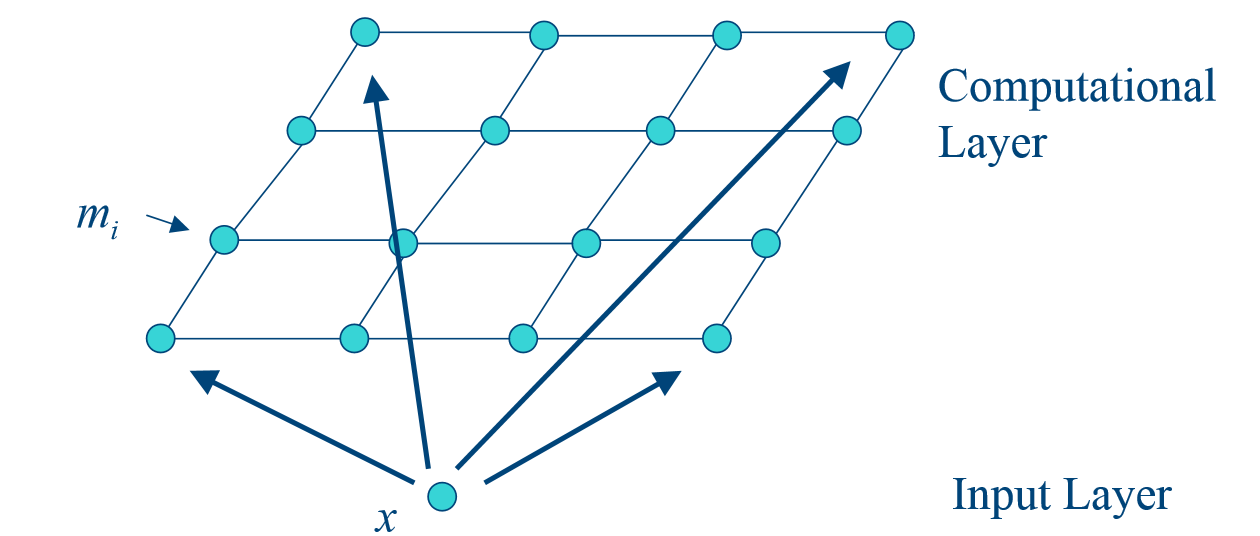
\includegraphics[width=6in,height=3in,keepaspectratio=true]{SOM1.png}
	\caption{Kiến trúc SOM}
  \end{figure}
  \subsubsection{Các thành phần}
  \begin{enumerate}
    \item Tập huấn luyện: 
    Đầu vào bao gồm một tập dữ liệu huấn luyện nhiều phần tử. Mỗi phần tử là một
    Vector có n chiều, và bao gồm p phần tử:
    \[ 
    \begin{bmatrix}
    x_{11} & x_{12} & \dots & x_{1n}\\
    x_{21} & x_{22} & \dots & x_{2n}\\
    \vdots & \vdots & \ddots & \vdots\\
    x_{p1} & x_{p2} & \dots & x_{pn}\\
    \end{bmatrix}
     \]
     \item Bản đồ các neuron: 
     Bản đồ một hoặc hai chiều với thành phần là các neuron với trọng số là một
     Vector có số chiều bằng với phần tử đầu vào
     \[ 
     \begin{bmatrix}
    w_{11} & w_{12} & \dots & w_{1n}\\
    w_{21} & w_{22} & \dots & w_{2n}\\
    \vdots & \vdots & \ddots & \vdots\\
    w_{q1} & w_{q2} & \dots & w_{qn}\\
    \end{bmatrix}
      \]
      Các neuron sẽ hình thành các cụm của bản đồ với mỗi cụm đại diện cho sự tương đồng thuộc tính của các phần tử trong tập huấn luyện. Mỗi cụm bao gồm một hoặc nhiều neuron đại diện. Số neuron được tạo ra ban đầu có thể nhỏ hơn, bằng hoặc lớn hơn số chiều của phần tử đầu vào nhưng phải nhỏ hơn tổng số phần tử của tập huấn luyện.
     \end{enumerate}
   \subsubsection{Các quá trình hình thành thuật toán}
   	 Quá trình tự tổ chức liên quan đến bốn quá trình chính:
   	 \begin{enumerate}
   	 \item Khởi tạo
   	 \begin{itemize}
   	   \item Chọn số lượng neuron thích hợp và số chiều của bản đồ   
   	   \item Tất cả các trọng số kết nối được khởi tạo với giá trị ngẫu nhiên
   	   nhỏ.
   	 \end{itemize}
   	 \begin{figure}[h!]
  	    \centering
	    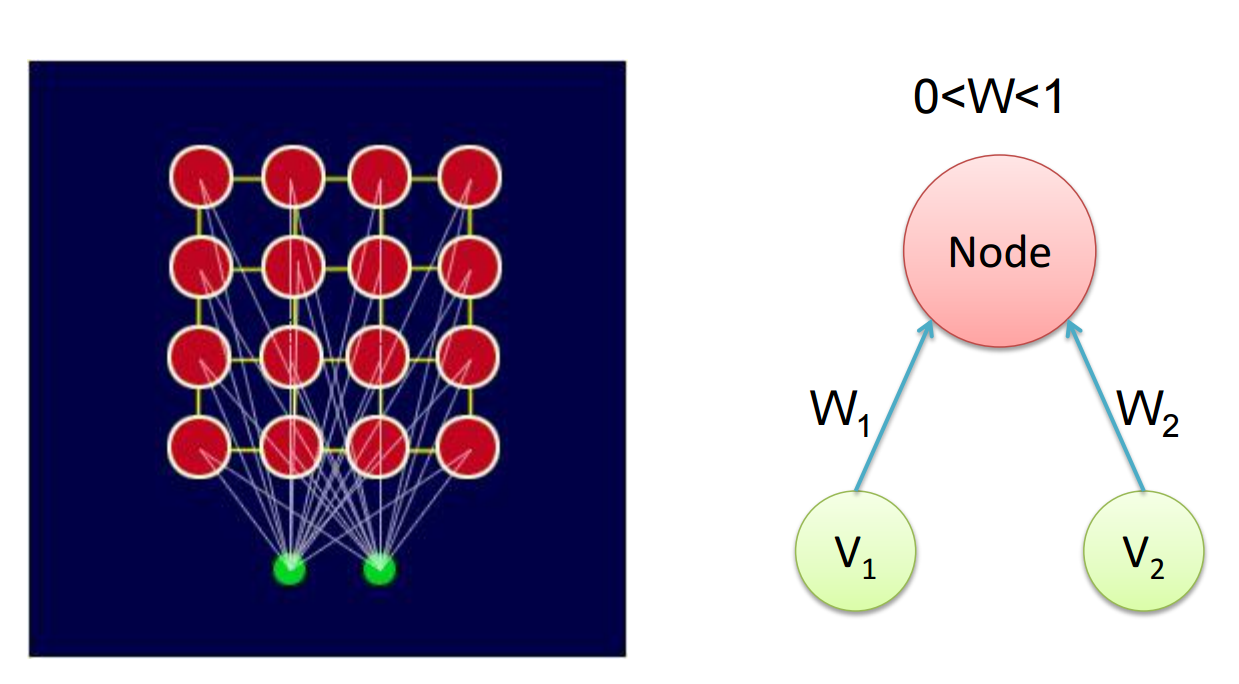
\includegraphics[width=5.5in,height=3.5in,keepaspectratio=true]{SOM2.png}
	    \caption{Khởi tạo SOM}
     \end{figure}
     \item Cạnh tranh\\
     Đối với mỗi mẫu đầu vào, các neuron tính toán giá trị tương ứng của một hàm biệt thức (discriminant function) cung cấp cơ sở cho sự cạnh tranh. Các neuron đặc biệt với giá trị nhỏ nhất của hàm biệt thức được tuyên bố là neuron chiến thắng (winning neuron).
     \item Hợp tác\\
     Các neuron giành chiến thắng xác định các vị trí không gian topo của neuron bị kích thích, do đó cung cấp cơ sở cho việc hợp tác giữa các neuron lân cận.
     \item Thích ứng\\
   	   Các neuron bị kích thích giảm giá trị trọng số về hàm biệt thức liên quan đến mô hình đầu vào thông qua điều chỉnh phù hợp của trọng số kết nối liên quan, như vậy là phản ứng của winning neuron trên các ứng dụng tiếp theo của một mô hình đầu vào tương tự được tăng cường.
   	 \end{enumerate}
	\subsubsection{Thuật toán SOM}
	Thuật toán SOM có thể được chia thành 7 bước:\\
	\textbf{Bước 1} : Số lượng neuron và trọng số của mỗi neuron được khởi tạo.
	Tương đương với quá trình khởi tạo.\\
	\textbf{Bước 2} : Một dữ liệu được chọn ngẫu nhiên từ tập dữ liệu huấn
	luyện và đưa vào mạng.\\
	\textbf{Bước 3} : Mỗi neuron trong mạng được kiểm tra để tính toán mà trọng số
	của nó gần giống như vector đầu vào. Các neuron chiến thắng thường được gọi là
	các đơn vị tốt nhất - Best Matching Unit (BMU). Đây là quá trình cạnh tranh.\\
	\textbf{Bước 4}: Bán kính ảnh hưởng của BMU được tính toán. Giá trị này ban đầu
là khá lớn. Thông thường nó được thiết lập để được bán kính của mạng, giảm dần
từng bước lặp của thuật toán.\\
	\textbf{Bước 5} : Bất kỳ các neuron lân cận được tìm thấy trong vòng bán kính ảnh hưởng của BMU đã tính trong bước 4 được điều chỉnh để làm cho chúng giống như các vector đầu vào. Càng nhiều neuron gần BMU, càng có nhiều trọng số được thay đổi (quá trình cộng tác).\\
	\textbf{Bước 6}: Lặp lại bước 2 với N vòng lặp.\\
	\textbf{Bước 7}: Sau khi kết thúc N vòng lặp, bản đồ đã được định hình thành
	với số cụm nhất định. Mỗi cụm đại diện bởi một hoặc nhiều neuron. Sau đó ta sẽ đưa các phần
tử của tập huấn luyện vào. Nếu neuron nào gần với phần tử đầu vào nhất thì phần
tử đầu vào sẽ thuộc cụm của neuron đó. Sau khi đưa tất cả các phần tử của tập
huấn luyện vào, các phần tử sẽ thuộc vào các cụm. Như vậy ta đã tiến hành phân
cụm thành công các phần tử của tập huấn luyện.     
	\subsubsection{Các quá trình thực hiện} 
	\begin{enumerate}
	  \item Quá trình cạnh tranh - The Competitive Process
	  \begin{itemize}
	    \item Nếu không gian đầu vào là D chiều (tức là D đơn vị đầu vào), có thể viết các
	  mẫu đầu vào như $x=\{x_i\::\:i=1,\dots,D\} $ và trọng số wj của neuron trong
	  lớp tính toán có thể được viết $w_j=\{w_i\::j=1,\dots,N;\:i=1,\dots,D\} $
	  trong đó N là tổng số neuron.
	  \item Sau đó chúng tôi có thể xác định chức năng biệt thức của
	  chúng tôi là khoảng cách Euclide bình phương giữa các vector đầu vào x và wj vector trọng số cho mỗi neuron j
	  \[ d_j(x) = \sum_{i=1}^D (x_i - w_{ji})^2 \]
	  \item Phương trình được tính bằng công thức khoảng cách Euclide bình phương
	  vì ta không quan tâm đến khoảng cách thực tế từ đầu vào. Chúng ta chỉ cần một số loại quy mô thống nhất để so sánh mỗi nút với vector đầu vào. Nói cách khác, các neuron có trọng số vector gần nhất với vector đầu vào được xác định là winning neuron.
	  \item Bằng cách này, không gian đầu vào liên tục có thể được ánh xạ vào không gian đầu ra rời rạc của neuron của một quá trình đơn giản của cuộc cạnh tranh giữa các neuron.
	  \end{itemize}
	  \item Quá trình hợp tác - The Cooperative Process\\
	  Trong các nghiên cứu sinh học thần kinh chúng ta thấy rằng có sự tương tác
	  bên trong một tập hợp các neuron bị kích thích. Khi một neuron hoạt động, các
	  neuron lân cận của nó có xu hướng dễ kích thích hơn so với những neuron ở
	  xa.
	  Có một topo lân cận phân rã theo khoảng cách. Chúng ta áp dụng lý thuyết đó
	  vào SOM với công thức
	  \[ T_{j,I(x)}=e^{-\frac{S_{j,I(x)}^2}{2\sigma^2}} \]
	  \begin{itemize}
	    \item $T_{j,I(x)}$ sử dụng để xác định các neuron gần với winning neuron
	    nhiều hơn các neuron khác nằm ngoài bán kính ảnh hưởng. Các neuron bên
	    ngoài bán kính ảnh hưởng được bỏ qua hoàn toàn.
	    \item $I(x)$ là vị trí của winning neuron. Điều này có một số đặc tính quan
	    trọng: nó là tối đa tại các neuron chiến thắng, nó là đối xứng về neuron đó, nó
	    làm giảm về giá trị 0 khi khoảng cách đi đến vô cùng, và nó không di chuyển 
	    (nghĩa là độc lập với vị trí của các neuron chiến thắng).
	    \item Trong đó $\sigma$ là bán kính ảnh hưởng của neuron
	    \[ \sigma(t) = \sigma_0 e^{\frac{-t}{\lambda}} \]
	    \tab t: vòng lặp hiện tại\\
	    \tab $\lambda$: hằng số = số vòng lặp / kích thước bản đồ $\sigma_0$. Giá
	    trị gần như là tùy ý. Bất kỳ giá trị hằng số nào cũng có thể được lựa chọn.
	    Tuy nhiên nó phụ thuộc trực tiếp vào kích thước bản đồ và số lần lặp để
	    thực hiện.\\
	    \tab $\sigma_0$: bán kính ảnh hưởng của neuron tại thờ điểm $t_0$ 
	  \end{itemize}
	  Một thuộc tính đặc biệt của SOM là $\sigma$ kích thước của bán kính ảnh hưởng
	  cần phải giảm theo thời gian. Một hàm thời gian phụ thuộc phổ biến là một
	  phân rã theo hàm số mũ.\\\\
	  Tại t = 0 giá trị là lớn nhất. Khi t (số lần lặp hiện hành) tăng lên,
	  giá trị tiệm cận bằng không. Đây chính là điều chúng ta muốn. Bán kính bắt
	  đầu như bán kính của mạng tinh thể, khi tiệm cận bằng không, lúc đó bán kính chỉ đơn giản là nút BMU\\
	  $S_{j,I(x)}$ là khoảng cách Euclid từ neuron lân cận đến winning neuron
	  \item Quá trình thích ứng - The Adaptive Process\\
	  Không phải chỉ có winning neuron được cập nhật trọng số mà các neuron lân cận
	  cũng được cập nhật. Trong thực tế, phương trình cập nhật trọng số thích hợp
	  là 
	  \[ \Delta w_{ji} = \eta(t).T_{j,I(x)} . (x_i - w_{ji})  \]
	  \[ w_{ji} = w_{ji} + \Delta w_{ji} \]
	  $\eta(t)$: tốc độ học tập - learning rate. Với $\eta(t+1) = \alpha
	  \eta(t)^{k/k_{max}}$ trong đó $0 \leq \alpha \leq 1$ quyết định lượng giảm
	  tốc độ học, k là số lần lặp của thuật toán đã được chạy, và $k_{max}$ là
	  thông số khi muốn việc học dừng lại.\\\\ 
	  Mỗi lần cập nhật trọng số học tập là để di chuyển các vector trọng số $w_i$
	  của winning neuron và các neuron lân cận về phía vector đầu vào x. Quá trình lặp
	  đi lặp lại của dữ liệu huấn luyện do đó dẫn đến trật tự topo.\\\\ 
	  Có hai giai đoạn mang tính chất của quá trình thích nghi này:
	  \begin{itemize}
	    \item Thứ tự hoặc giai đoạn tự tổ chức (Ordering or self-organizing phase )
	    - trong đó thứ tự topo của vector trọng số diễn ra. Thông thường điều này
	    sẽ mất là 1000 lần lặp lại các thuật toán SOM, và xem xét cẩn thận cần phải
	    được đưa ra để lựa chọn bán kính ảnh hưởng và tham số tốc độ học.
	    \item Hội tụ - trong đó các bản đồ feature được tinh chỉnh và đến khi cung
	    cấp một lượng thống kê chính xác về không gian đầu vào. Thông thường các số lần lặp lại trong giai đoạn này sẽ có ít nhất hơn 500 lần số lượng neuron trong mạng, và một lần nữa các thông số phải được lựa chọn cẩn thận.
	  \end{itemize}
	\end{enumerate}
\subsection{Ví dụ của SOM}
\begin{figure}[h!]
  \begin{minipage}{0.4\textwidth}
	\centering
    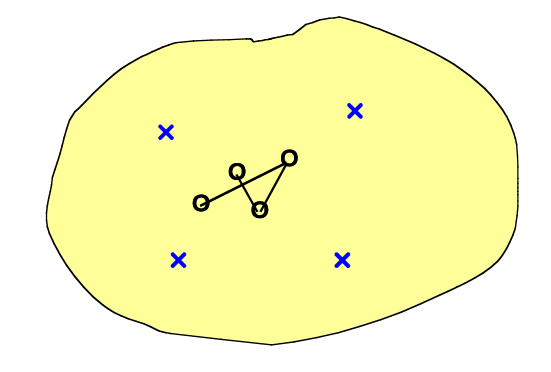
\includegraphics[width=1\textwidth,keepaspectratio=true]{SOM6.png}
    \caption{Bước 1: Khởi tạo giá trị bảng đầu}
  \end{minipage}
  ~
  \begin{minipage}{0.1\textwidth}
  \end{minipage}
  ~
  \begin{minipage}{0.5\textwidth}
  Giả sử ta có bốn điểm dữ liệu trong không gian đầu vào hai chiều liên tục, và muốn đưa vào bốn điểm trong một không gian đầu ra một chiều rời rạc. Các nút đầu ra (neuron) được đưa các điểm trong không gian đầu vào (vòng tròn). Trọng số ban đầu được chọn ngẫu nhiên là vòng tròn tại các vị trí ngẫu nhiên trong trung tâm của không gian đầu vào. 
  \end{minipage}
\end{figure}
\begin{figure}[h!]
  \begin{minipage}{0.4\textwidth}
	\centering
    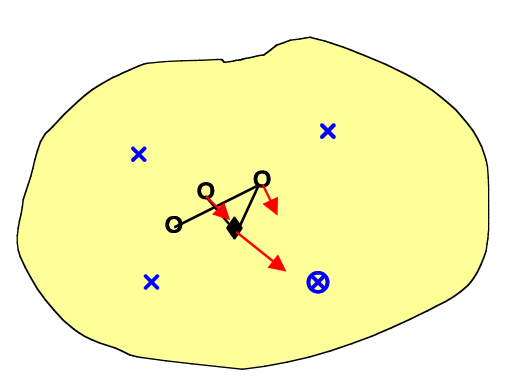
\includegraphics[width=1\textwidth,keepaspectratio=true]{SOM3.png}
    \caption{Bước 2: Đưa giá trị đầu vào học}
  \end{minipage}
  ~
  \begin{minipage}{0.1\textwidth}
  \end{minipage}
  ~
  \begin{minipage}{0.5\textwidth}
  Ta chọn ngẫu nhiên một trong những điểm dữ liệu cho vào học (kí hiệu là vòng tròn bao quanh dấu x). Các điểm đầu ra gần nhất đại diện cho các neuron chiến thắng (tứ giác được tô đen). Đó là winning neuron đang di chuyển về phía điểm dữ liệu bằng lượng nhất định, và hai neuron lân cận di chuyển bởi một lượng nhỏ hơn (mũi tên).
  \end{minipage}
\end{figure}
\begin{figure}[h!]
  \begin{minipage}{0.4\textwidth}
	\centering
    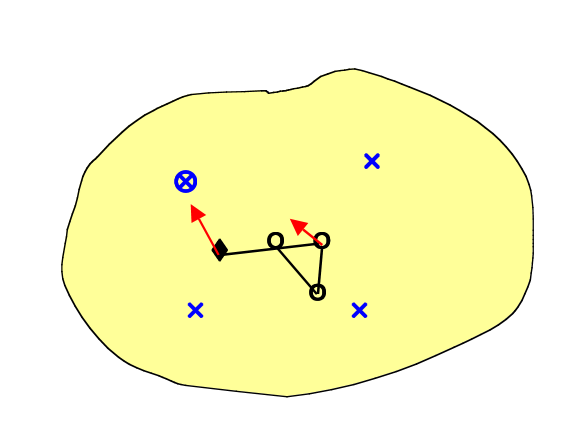
\includegraphics[width=1\textwidth,keepaspectratio=true]{SOM4.png}
    \caption{Bước 3: Học giá trị tiếp theo}
  \end{minipage}
  ~
  \begin{minipage}{0.1\textwidth}
  \end{minipage}
  ~
  \begin{minipage}{0.5\textwidth}
  Tiếp tục chọn ngẫu nhiên một điểm dữ liệu cho vào học (qua trong vòng tròn).
  Winning neuron đang tiến về điểm đầu vào bằng lượng nhất định, và neuron lân cận di chuyển bởi một lượng nhỏ hơn (mũi tên).
  \end{minipage}
\end{figure}
 \vfill
\begin{figure}[h!]
  \begin{minipage}{0.4\textwidth}
	\centering
    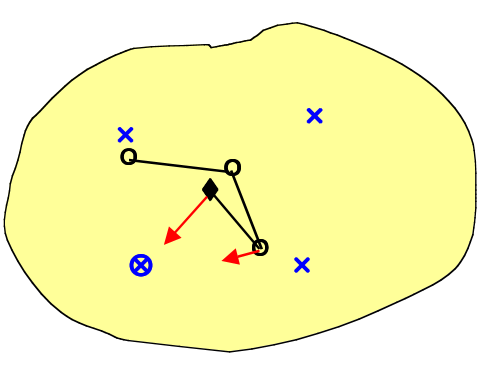
\includegraphics[width=1\textwidth,keepaspectratio=true]{SOM5.png}
    \caption{Bước 4: Tiếp tục cho các giá trị vào học}
  \end{minipage}
  ~
  \begin{minipage}{0.6\textwidth}
  Tiếp tục chọn ngẫu nhiên một điểm dữ liệu cho học (qua trong vòng tròn).
  Winning neuron đang tiến về điểm dữ liệu bằng một lượng nhất định, và một
  trong những neuron láng giềng di chuyển bởi một số lượng nhỏ hơn (mũi
  tên).
  Cuối cùng toàn bộ lưới được xác định để đại diện cho không gian đầu vào.
  \end{minipage}
\end{figure}

\subsection{Ứng dụng của SOM}
  SOM thường được sử dụng làm công cụ trực quan. Nó giúp chúng ta hình dung dễ
  dàng về mối quan hệ giữa khối lượng lớn dữ liệu.\\ 
\begin{figure}[h!]
	\centering
    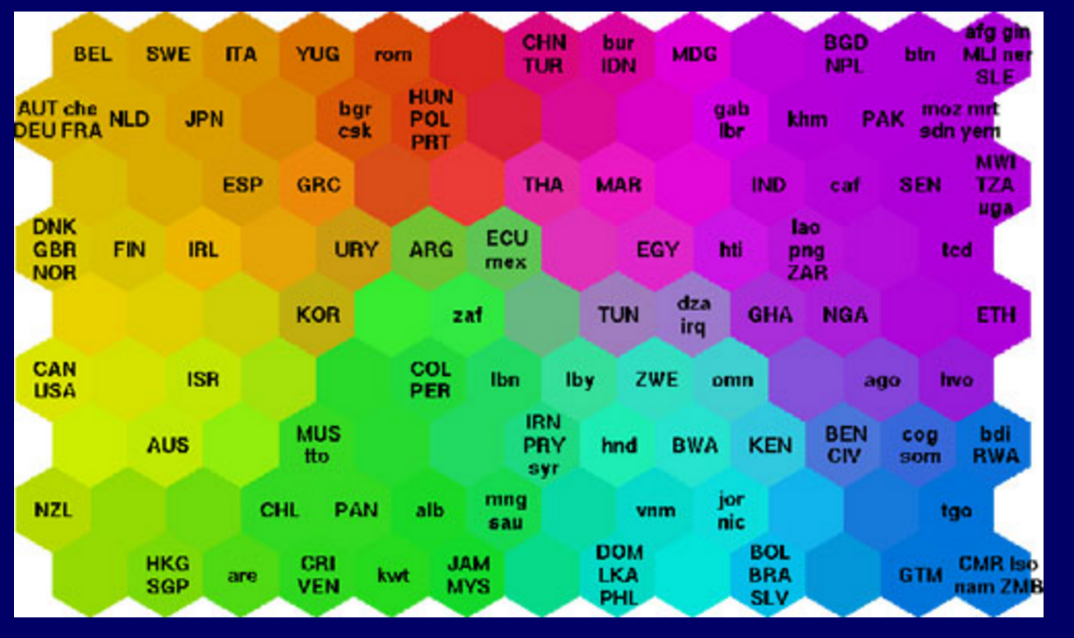
\includegraphics[width=5in,keepaspectratio=true]{SOM_ex1.png}
    \caption{Biểu đồ thể hiện chất lượng cuộc sống các quốc gia}
\end{figure}
SOM đã được sử dụng để phân loại dữ liệu thống kê mô tả khác nhau chất lượng của
cuộc sống theo các yếu tố như tình trạng sức khỏe, dinh dưỡng, các dịch vụ giáo
dục, \ldots. Các quốc gia có chất lượng cuộc sống với các yếu tố tương tự cùng
nhóm nhau. Các quốc gia có chất lượng cuộc sống tốt hơn nằm phía trên bên trái và các nước nghèo khó nhất nằm ở phía dưới bên phải. Lưới lục giác là một ma trận khoảng cách thống nhất, thường được biết đến như một U-ma trận. Mỗi hình lục giác đại diện cho một nút trong SOM\\
Ngoài ra còn có một số ứng dụng khác như phân loại hình ảnh hay màu sắc.
\begin{figure}[h!]
	\centering
    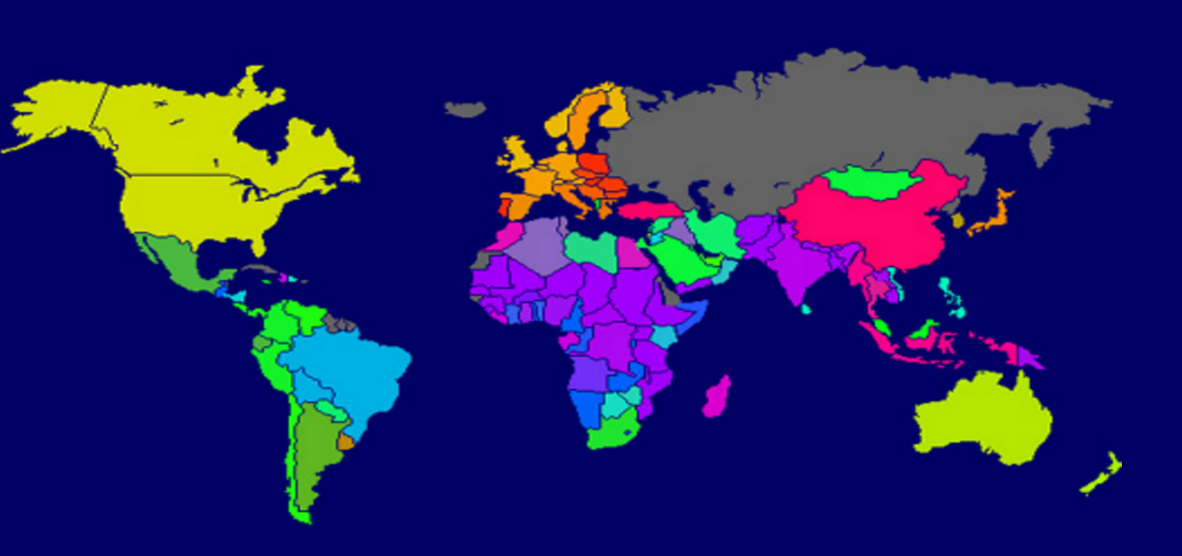
\includegraphics[width=5in,keepaspectratio=true]{SOM_ex2.png}
    \caption{Bản đồ chất lượng cuộc sống thế giới}
\end{figure}